\documentclass{article}

% if you need to pass options to natbib, use, e.g.:
%     \PassOptionsToPackage{numbers, compress}{natbib}
% before loading neurips_2018

% ready for submission
% \usepackage{neurips_2018}

% to compile a preprint version, e.g., for submission to arXiv, add add the
% [preprint] option:
 % \usepackage[preprint]{neurips_2018}

% to compile a camera-ready version, add the [final] option, e.g.:
 \usepackage[final]{neurips_2019}
% to avoid loading the natbib package, add option nonatbib:
%     \usepackage[nonatbib]{neurips_2018}
\usepackage{graphicx}
\usepackage[utf8]{inputenc} % allow utf-8 input
\usepackage[T1]{fontenc}    % use 8-bit T1 fonts
\usepackage{hyperref}       % hyperlinks
\usepackage{url}            % simple URL typesetting
\usepackage{booktabs}       % professional-quality tables
\usepackage{amsfonts}       % blackboard math symbols
\usepackage{nicefrac}       % compact symbols for 1/2, etc.
\usepackage{microtype}      % microtypography
\usepackage{amsmath}
\usepackage{bm}
\usepackage{subfig}
\usepackage[english]{babel}
\usepackage{algorithm}
\usepackage{algorithmic}
\usepackage{amsthm}
\usepackage{dsfont}
\usepackage{comment}
\usepackage{enumitem}
\usepackage{multirow}



\usepackage{appendix}
\newtheorem{theorem}{Theorem}
\newtheorem{lemma}{Lemma}
\newtheorem{exam}{Example}
\newtheorem{prop}{Proposition}
\newtheorem{property}{Property}
\input macros.tex


\newcommand*{\KeepStyleUnderBrace}[1]{%f
  \mathop{%
    \mathchoice
    {\underbrace{\displaystyle#1}}%
    {\underbrace{\textstyle#1}}%
    {\underbrace{\scriptstyle#1}}%
    {\underbrace{\scriptscriptstyle#1}}%
  }\limits
}
\usepackage{xr}
\usepackage{mathtools}
\mathtoolsset{showonlyrefs}
\renewcommand{\thefigure}{{S\arabic{figure}}}%
\renewcommand{\thetable}{{S\arabic{table}}}%
\renewcommand{\figurename}{{Supplementary Figure}}    
\renewcommand{\tablename}{{Supplementary Table}}    
\setcounter{figure}{0}   
\setcounter{table}{0}  




\externaldocument{tensor_block_model}

\title{Supplements for ``Multiway clustering via tensor block models''}


%\author{%
%Yuchen Zeng \\
%University of Wisconsin -- Madison\\
 %\texttt{yzeng58@wisc.edu} \\
%\And
%Miaoyan Wang \\
%University of Wisconsin -- Madison\\
%\texttt{miaoyan.wang@wisc.edu} \\
%}

\begin{document}

\maketitle

\vspace{-2cm}
\begin{appendices}
\section{Proofs}
\subsection{Stochastic tensor block model}
The following property shows that Bernoulli distribution belongs to the sub-Gaussian family with a subgaussianity parameter $\sigma$ equal to $1/4$.
\begin{property}
Suppose $x \sim \text{Bernoulli}(p)$, then $x\sim \text{sub-Gaussian}({1\over 4})$.
\end{property}
\begin{proof} For all $\lambda \in \mathbb{R}$, we have
\[
\ln(\mathbb{E}(e^{\lambda(x-p)})=\ln\left(pe^{\lambda(1-p)} +(1-p)e^{-p\lambda}\right)=-p\lambda +\ln (1+pe^\lambda  -p)\leq {\lambda ^2\over 8}.
\]
Therefore $\mathbb{E}(e^{\lambda (x-p)})\leq e^{\lambda^2(1/4)/2}$.
\end{proof}

\subsection{Proof of Proposition~\ref{prop:factors}}
\begin{proof}
Let $\mathbb{P}_{\Theta}$ denotes the (either Gaussian or Bernoulli) tensor block model, where $\Theta=\tC \times_1\mM_1\times_2\cdots\times_K\mM_K$ parameterizes the mean tensor. Since the mapping $\Theta\mapsto\mathbb{P}_{\Theta}$ is one-to-one, $\Theta$ is identifiable. Now suppose that $\Theta$ can be decomposed in two ways, $\Theta=\Theta(\{\mM_k\}, \tC)=\Theta(\{\tilde \mM_k\}, \tilde \tC)$. Based on the Assumption~\ref{ass:core}, we have
\begin{equation}\label{eq:equality}
\Theta=\tC \times_1\mM_1\times_2\cdots\times_K\mM_K=\tilde \tC \times_1\tilde \mM_1\times_2\cdots\times_K\tilde  \mM_K,
\end{equation}
where $\tC$, $\tilde \tC\in\mathbb{R}^{R_1\times \cdots \times R_K}$ are two irreducible cores, and $\mM_k,\tilde \mM_k\in\{0,1\}^{R_k\times d_k}$ are membership matrices for all $k\in[K]$. We will prove by contradiction that $\mM_k$ and $\tilde \mM_k$ induce the same partition of $[d_k]$, for all $k\in[K]$. 

Suppose the above claim does not hold. Then there exists a mode $k\in[K]$ such that the $\mM_k, \tilde \mM_k$ induce two different partitions of $[d_k]$. Without loss of generality, we assume $k=1$. The definition of partition implies that there exists a pair of indices $i\neq j$, $i,j\in[d_1]$, such that, $i,j$ belong to the same cluster based on $\mM_1$, but they belong to different clusters based on $\tilde \mM_1$. Let $\tA\neq \tB, \tA, \tB \subset[d_1]$ respectively denote the  clusters that $i$ and $j$ belong to, based on $\tilde \mM_1$. The left-hand side of \eqref{eq:equality} implies
\begin{equation}\label{eq:cluster1}
\Theta_{i,i_2,\ldots,i_K}=\Theta_{j,i_2,\ldots,i_K},\quad \text{for all } (i_2,\ldots,i_K)\in[d_2]\times\cdots\times [d_K].
\end{equation}
 On the other hand, \eqref{eq:equality} implies
\begin{equation}\label{eq:cluster2}
\Theta_{i,i_2,\ldots,i_K}=\Theta_{k,i_2,\ldots,i_K},\quad \text{for all } k\in \tA \text{ and all }(i_2,\ldots,i_K)\in[d_2]\times\cdots\times [d_K],
\end{equation}
and
\begin{equation}\label{eq:cluster3}
\Theta_{j,i_2,\ldots,i_K}=\Theta_{k,i_2,\ldots,i_K},\quad \text{for all } k\in \tB \text{ and all }(i_2,\ldots,i_K)\in[d_2]\times\cdots\times [d_K].
\end{equation}

Combining~\eqref{eq:cluster1}, \eqref{eq:cluster2} and \eqref{eq:cluster3}, we have
\begin{equation}\label{eq:same}
\Theta_{i,i_2,\ldots,i_K}=\Theta_{k,i_2,\ldots,i_K},\quad \text{for all } k\in \tA\cup \tB \text{ and all }(i_2,\ldots,i_K)\in[d_2]\times\cdots\times [d_K].
\end{equation}
Equation~\eqref{eq:same} implies that $\tA$ and $\tB$ can be merged into one cluster. This contradicts the irreducibility assumption of the core tensor $\tilde \tC$. Therefore, $\mM_1$ and $\tilde \mM_1$ induce a same partition of $[d_1]$, and thus they are equal up to permutation of cluster labels. The proof is now complete. 
\end{proof}

%Based on the definition of membership matrix, $\mM_k\mM_k'=\text{diag}(R_1,\ldots,R_K)$ is a diagonal matrix and thus invertible. Multiplying $\mM_k'(\mM_k\mM_k')^{-1}$ to the $k$-th mode of Equation~\eqref{eq:equality} gives
%\begin{equation}\label{eq:core}
%\tC=\tilde \tC \times_1\left(\tilde \mM_1 \mM_1'(\mM_1\mM_1')^{-1}\right) \times_2\cdots\times_K \left(\tilde   \mM_K \mM_K'(\mM_K\mM_K')^{-1}\right).
%\end{equation}
%Define $\mB_k=\tilde \mM_k \mM_k'(\mM_k\mM_k')^{-1}$. It remains to show that each $\mB_k$ is a permutation matrix. 


%Now, the definition of membership matrix implies that $\mB_k$ is a column-wise normalized confusion matrix, where its $(r,s)$-th entry is
%\[
%\mB_{k,(r,s)}={ \#\{i\in[d]: \tilde \mM_k(i)=r, \mM_k(i)=s\}\over \#\{i\in[d]: \mM_k(i)=s\}}\in[0,1],
%\] 
%where $\#$ denotes the cardinality size of the set. Plugging $\mB_k$ back to the Equations~\eqref{eq:equality} and~\eqref{eq:core} yields
%\begin{equation}\label{eq:cluster}
%\tilde \tC \times_1 \left(\mB_1\mM_1\right) \times_2 \cdots\times_K \left(\mB_K\mM_K\right)=\tilde \tC \times_1 \tilde \mM_1 \times_2 \cdots\times_K \tilde \mM_K.
%\end{equation}
%Both sides of the above expression represent a block tensor with a same core. Let us consider the mode-1 structure first. Based on the Assumption~\ref{ass:core}, $\mB_1\mM_1$ has full row rank. Furthermore, the mode-$1$ partition is determined by $\mM_1$, because multiplying a $R_1$-by-$R_1$ confusion matrix $B_1$ will not change the cluster allocation. On the right-hand hand, the mode-$1$ partition is determined by $\tilde \mM_1$. Therefore the partition encoded in $\mM_1$ is the same as that in $\tilde \mM_1$. Equivalently, $\mB_1$ must be a permutation matrix. The proof is complete by applying the same argument to all $k\in[K]$. 
%\subsection{Proof of Theorem~\ref{thm:main}}
%We first present three lemmas that will be used in the proof of Theorem~\ref{thm:main}. 
%\begin{lemma} 
%\end{lemma}
\subsection{Proofs of Theorems~\ref{thm:main} and~\ref{thm:partition}}
The following lemma is useful for the proof of Theorem~\ref{thm:main}.
\begin{lemma} \label{lem:high}
Suppose $\tY=\trueT+\tE$ with $\trueT\in\tP$. Let $\hat \Theta=\arg\min_{\Theta \in \tP}\FnormSize{}{\hat \Theta-\tY}^2$ be the least-square estimator of $\trueT$. We have
\[
\FnormSize{}{\hat \Theta-\trueT}\leq 2\sup_{\mu \in { \tP-\tP'\over |\tP-\tP'|}}\langle \mu, \tE \rangle,
\]
\end{lemma}
where $\tP-\tP'=\{\Theta-\Theta'\colon \Theta, \Theta'\in \tP\}$ and $\tS/|\tS|=\{s/\vnormSize{}{s}\colon s\in \tS\}$.
\begin{proof} Based on the definition of least-square estimator, we have
\begin{equation}\label{eq:least}
\FnormSize{}{\hat \Theta-\tY}^2\leq \FnormSize{}{\trueT-\tY}^2.
\end{equation}
Combining~\eqref{eq:least} with the fact 
\begin{align}
\FnormSize{}{\hat \Theta -\tY}^2&=\FnormSize{}{\hat \Theta-\trueT+\trueT-\tY}^2\\
&=\FnormSize{}{\hat \Theta-\trueT}^2+\FnormSize{}{\trueT-\tY}^2+2\langle \hat \Theta-\trueT, \trueT-\tY\rangle,
\end{align}
yields
\[
\FnormSize{}{\hat \Theta-\trueT}^2\leq 2\langle \hat \Theta-\trueT, \tY-\trueT\rangle=2\langle \hat \Theta-\trueT, \tE\rangle.
\]
Dividing each side by $\FnormSize{}{\hat \Theta-\trueT}$, we have
\[
\FnormSize{}{\hat \Theta-\trueT}\leq 2\left \langle {\hat \Theta-\trueT \over \FnormSize{}{\hat \Theta-\trueT}}, \tE\right \rangle.
\]
The desired inequality follows by noting ${\hat \Theta-\trueT \over \FnormSize{}{\hat \Theta-\trueT}}\in {\tP-\tP'\over |\tP-\tP'|}$. 
\end{proof}

\begin{proof}[Proof of Theorem~\ref{thm:main}]
To study the performance of the least-square estimator $\hat \Theta$, we need to introduce some additional notation. We view the membership matrix $\mM_k$ as an onto function $\mM_k\colon [d_k]\mapsto [R_k]$. With a little abuse of notation, we still use $\mM_k$ to denote the mapping function and write $\mM_k\in R_k^{d_k}$ by convention. We use $\mM=\{\mM_k\}_{k\in[K]}$ to denote the collection of $K$ membership matrices, and write $\tM=\{\mM \colon \text{$\mM$ is the collection of membership matrices $\mM_k$'s}\}$. For any set $J$, $|J|$ denotes its cardinality. Note that $|\tM|\leq \prod_k R_k^{d_k}$, because each $\mM_k$ can be identified by a partition of $[d_k]$ into $R_k$ disjoint non-empty sets. 

For ease of notation, we define $d=\prod_k d_k$ and $R=\prod_k R_k$. We sometimes identify a tensor in $\mathbb{R}^{d_1\times \cdots \times d_K}$ with a vector in $\mathbb{R}^d$. By the definition of the parameter space $\tP$, the element $\Theta\in \tP$ can be equivalently identified by $\Theta=\Theta(\mM, \mC)$, where $\mM\in \tM$ is the collection of $K$ membership matrices and $\mC=\text{vec}(\tC)\in\mathbb{R}^R$ is the core tensor. Note that, for a fixed clustering structure $\mM$, the space consisting of $\Theta=\Theta(\mM,\cdot)$ is a linear space of dimension $R$. 



%Correspondingly, we use $\mM_k(i_k)$ to denote the cluster label for the element $i_k\in[d_k]$, and $\mM^{-1}_k(r_k)$ the group of elements in cluster $r_k\in[R_k]$.

Now consider the least-square estimator
\[
\hat \Theta=\argmin_{\Theta\in\tP}\{-2\langle \tY, \Theta\rangle+\FnormSize{}{\Theta}^2 \}=\argmin_{\Theta\in\tP}\{\FnormSize{}{\tY-\Theta}^2 \}.
\]
Based on the Lemma~\ref{lem:high},
\begin{align}
\FnormSize{}{\hat \Theta-\trueT}&\leq 2\sup_{\Theta\in\tP} \sup_{\Theta'\in \tP} \Big\langle {\Theta-\Theta'\over \FnormSize{}{\Theta-\Theta'}}, \tE \Big\rangle\\
&\leq 2\sup_{\mM, \mM' \in \tM}\sup_{\mC, \mC' \in \mathbb{R}^R}\Big\langle {\Theta(\mM, \mC)-\Theta'(\mM', \mC')\over \FnormSize{}{\Theta(\mM, \mC)-\Theta' (\mM', \mC')}}, \tE \Big\rangle.
\end{align}
%where $\tP-\Theta=\{\Theta'-\Theta: \Theta' \in \tP\}$ denotes the shifted set for a given $\Theta$. 

By union bound, we have, for any $t>0$,
\begin{align}
\mathbb{P}\left(\FnormSize{}{\hat \Theta-\trueT} > t\right)&\leq \mathbb{P}\left(\sup_{\mM, \mM'\in \tM}\sup_{\mC, \mC'\in \mathbb{R}^R} \left|\Big\langle {\Theta-\Theta'\over \FnormSize{}{\Theta-\Theta'}}, \ \tE\Big\rangle\right|>{t\over 2}\right)\\
&\leq \sum_{\mM, \mM'\in \tM}\mathbb{P}\left(\sup_{\mC'\in \mathbb{R}^R}\sup_{\mC\in \mathbb{R}^R}\left|\Big\langle {\Theta-\Theta'\over \FnormSize{}{\Theta-\Theta'}},\ \tE\Big\rangle \right|\geq {t\over 2}\right)\\
&\leq |\tM|^2C_1^R\exp\left(-{C_2 t^2\over 32\sigma^2}\right)\\
&=\exp\left(2\sum_kd_k\log R_k+C_1\prod_k R_k-{C_2t^2\over 32\sigma^2}\right),
\end{align}
for two universal constants $C_1, C_2>0$. Here the third line follows from~\cite{rigollet2015high} (Theorem 1.19) and the last line uses the factor $|\tM|\leq \prod_k R_k^{d_k}$ and $R=\prod_k R_k$. Choosing $t=C\sigma\sqrt{\prod_k R_k+\sum_k d_k\log R_k}$ yields the desired bound. 
\end{proof}

%\begin{lemma}  With very high probability
%\[
%\mnormSize{}{\hat \tC-\trueC}\to 0
%\]
%\end{lemma}


\begin{proof}[Proof of Theorem~\ref{thm:partition}]
Let $\trueM, \hat \mM_k$ denote the true and estimated membership matrix in the mode $k$, respectively. It suffices to show that
\begin{equation}\label{CER}
\text{CER}(\hat \mM_k, \trueM)={1\over d_k}\sum_{i\in[d_k]}\mathds{1}\{\trueM(i)\neq \hat \mM_k(i)\} \to 0,\quad \text{for all }k \in[K]. 
\end{equation}
We provide the proof below for $k=1$; the proof for other modes is exactly the same. We use $\mj=(i_2,\ldots,i_K)$ to denote the tensor coordinates except the 1st mode. Define the gap between cluster means
\[
\delta=\min_{i\in[r_1]}\min_{\mj,\mj'\in[r_2]\times \cdots [r_K]}|\trueC(i,\mj)-\trueC(i,\mj')|.
\]
Note that $\delta>0$ from the Assumption~\ref{ass:core}. Based on a modified proof of Theorem~\ref{thm:main}, we have
\begin{equation}\label{eq:zero}
\mnormSize{}{\hat \Theta-\trueT}\to  0,\quad \text{as $d_{\min} \to \infty$},
\end{equation}
where $\mnormSize{}{\cdot}$ denotes the maximum absolute entry value in the tensor. Therefore, when $d_{\min}$ is sufficiently large,
\begin{equation}\label{eq:fact}
\mnormSize{}{\hat \Theta -\trueT} < {\delta\over 2}.
\end{equation}
The inequality~\eqref{eq:fact} implies that $\mM_1$ and $\mM_{\text{true},1}$ disagree at most $o(d_1)$ entries. Otherwise, there exist $O(d_1)$ pairs of indices $r,s\in[d_1]$, such that they belong to the same cluster in $\hat \Theta$, but they belong to different clusters in $\trueT$. Then, we have
\[
|\trueT_{,r,\mj}-  \trueT_{,s,\mj}|\leq  |\trueT_{,r,\mj}-\hat \Theta_{r,\mj}|+|\hat \Theta_{r,\mj}- \hat \Theta_{s,\mj}|+| \hat \Theta_{s,\mj}-\trueT_{,s,\mj}|<\delta,
\]
for all $\mj \in[d_2]\times \cdots \times [d_K]$. This contracts the definition of $\delta$. Therefore, the convergence~\eqref{CER} holds.  
\end{proof}

\subsection{Sparse estimator}
\begin{lemma}\label{prop:sparse}
Consider the regularized least-square estimation,
\begin{equation}\label{eq:opt}
\hat \Theta^{\text{sparse}}=\argmin_{\Theta\in \tP}\left\{\FnormSize{}{\tY-\Theta}^2+\lambda \normSize{}{\tC}_\rho
\right\},
\end{equation}
where $\tC=\entry{c_{r_1,\ldots,r_K}}\in\mathbb{R}^{R_1\times \cdots\times R_K}$ is the block-mean tensor, $\normSize{}{\tC}_\rho$ is the penalty function with $\rho$ being an index for the tensor norm, and $\lambda$ is the penalty tuning parameter. We have
\begin{equation}\label{eq:lasso}
\hat c^{\text{sparse}}_{r_1,\ldots,r_K}=
\begin{cases}
\hat c^{\text{ols}}_{r_1,\ldots,r_K}\mathds{1}\left\{|\hat c^{\text{ols}}_{r_1,\ldots,r_K} |\geq {\sqrt{\lambda \over n_{r_1,\ldots,r_K}}}\right\} & \text{if}\ \rho=0,\\
\text{sign}(\hat c^{\text{ols}}_{r_1,\ldots,r_K})\left( |\hat c^{\text{ols}}_{r_1,\ldots,r_K}|-{\lambda \over 2n_{r_1,\ldots,r_K}}  \right)_{+} &\text{if}\ \rho=1,
\end{cases}
\end{equation}
where $a_{+}=\max(a,0)$ and $\hat c^{\text{ols}}_{r_1,\ldots,r_K}$ denotes the ordinary least-square estimate as in Algorithm~\ref{alg:B}. 
\end{lemma}

\begin{proof}
We formulate the estimation of $\tC$ as a regularized least-square regression. Note that $\Theta\in\tP$ implies that
\[
\Theta=\tC\times_1\mM_1\times \cdots \times_K \mM_K.
\]
Define $\mX=\mM_1\otimes \ldots \otimes \mM_K\in \mathbb{R}^{d\times R}$, where $d=\prod_k d_k$ and $R=\prod_k R_k$, and ${\bm \beta}=\text{vec}(\tC)\in\mathbb{R}^R$. Here $\mX$ is a membership matrix that indicates the block allocation among tensor entries. Specifically, $\mX$ consists of orthogonal columns with $\mX^T\mX=\text{diag}(n_1,\ldots,n_R)$, where $n_r$ is the number of entries in the tensor block that corresponds to the $r$-th column of $\mX$.

For a given set of $\mM_k's$, the optimization~\eqref{eq:opt} with respect to $\tC$ is equivalent to a regularized linear regression with $\mY=\text{vec}(\tY)$ as the response and $\mX$ as the design matrix:
\begin{equation}\label{eq:opt}
L({\bm \beta})=\vnormSize{}{\mY-\mX \bm{\beta}}^2+\lambda\normSize{}{\bm{\beta}}_\rho.
\end{equation}
When $\lambda=0$ (no penalty), the minimizer is $\hat {\bm \beta}^{\text{ols}}=(\hat \beta^{\text{ols}}_1,\ldots,\hat \beta^{\text{ols}}_R)=(\mX^T\mX)^{-1}\mX^T\mY$, where $\hat \beta^{\text{ols}}_r={1\over n_r}\my_{\mr}\mathbf{1}^T_{n_r}$ for all $r\in[R]$.

{\bf Case 1: } $\rho=0$.\par
%Note that $\zeronorm{\boldsymbol{\beta}}$ takes on integer values in $\{1,2,\ldots, R\}$. We will find the optimal $L_1$ for different values of $L_2$. 
Note that $\mX$ induces a partition of indices $[d]$ into $R$ blocks. With a little abuse of notation, we use ${\mr}=\{i\in[d]:\mX(i)=r\}$ to denote the tensor indices that belong to the $r$th block, and use $\my_{\mr}\in\mathbb{R}^{n_r}$ to denote the corresponding tensor entries. By the orthogonality of $\mX$, we have
\begin{align}
L(\boldsymbol{\beta})&=\sum_{r=1}^R \vnormSize{}{\my_{\mr}-\beta_r\mathbf{1}_{n_r}}^2+\lambda \sum_{r=1}^R \mathds{1}{\{ \beta_r\neq 0\}}\\
&=\sum_{r=1}^R\KeepStyleUnderBrace{\left( \vnormSize{}{\my_{\mr}-\beta_r\mathbf{1}_{n_r}}^2+\lambda \mathds{1}{\{ \beta_r\neq 0\}}\right)}_{:=L_r(\beta_r)}
\end{align}
The optimization can be separated into each of $\beta_r$'s. For any $r\in[R]$, the sub-optimization $\min_{\beta_r}L_r(\beta_r)$ has a closed-form solution
\[
\min_{\beta_r} L_r(\beta_r)
=\begin{cases}
\my^T_{\mr}\my_{\mr}-n_r\left(\hat \beta_r^{\text{ols}}\right)^2+\lambda& \text{if $\hat \beta^{\text{ols}}_r\neq 0$,}\\
\my^T_{\mr}\my_{\mr}&\text{if $\hat \beta^{\text{ols}}_r=0$,}
\end{cases}
\]
with
\begin{equation}\label{eq:sparse}
\arg\min_{\beta_r} L_r(\beta_r)=
\begin{cases}
0\quad& \text{if $n_r\left(\hat \beta_r^{\text{ols}}\right)^2 \leq \lambda$},\\
\hat \beta_r^{\text{ols}} &\text{otherwise}.
\end{cases}
\end{equation}
Solution~\eqref{eq:sparse} can be simplified as $\hat \beta^{\text{sparse}}_r=\hat \beta^{\text{ols}}_r\mathds{1}\{|\hat \beta^{\text{ols}}_r| \leq \sqrt{\lambda \over n_r}\}$. The proof is complete by noting that $\hat c^{\text{sparse}}_{r_1,\ldots,r_R}=\hat \beta^{\text{sparse}}_r$ and $n_{r_1,\ldots,r_K}=n_r$ for all $(r_1,\ldots,r_K)\in[R_1]\times \cdots \times [R_K]$.



{\bf Case 2: } $\rho=1$.\par

Similar as in Case 1, we write the optimization~\eqref{eq:opt} as
\[
L({\bm \beta})=\sum_{r=1}^R\KeepStyleUnderBrace{\left(\vnormSize{}{\my_{\mr}-\beta_r\mathbf{1}_{n_r}}^2+\lambda |\beta_{r}|\right)}_{:=L_r(\beta_r)},
\]
where, with a little abuse of notation, we still use $L_r(\beta_r)$ to denote the sub-optimization. To solve $\argmin_{\beta_r}L_r(\beta_r)$, we use the properties of subderivative. Taking the subderivative with respect to $\beta_r$, we obtain
	
\begin{equation}
\frac{\partial L_r(\beta_r)}{\partial \beta_r} = 
\begin{cases}
2n_r\beta_r-2n_r\hat \beta^{\text{ols}}_r+\lambda &\mbox{if $\beta_r>0$,}\\
 [2n_r\beta_r-2\hat \beta^{\text{ols}}_r-\lambda, \ 2n_r\beta_r-\hat \beta^{\text{ols}}+\lambda]&\mbox{if $\beta_r=0$,}\\
2n_r\beta_r-2n_r\hat \beta^{\text{ols}}_r+\lambda &\mbox{if $\beta_r<0$.}\\
\end{cases}
\end{equation}
Because $\hat \beta^{\text{sparse}}_r$ minimizes $L_r(\beta_r)$ if and only if $0 \in \frac{\partial L_r(\beta_r)}{\partial \beta_j}$, we have:
\begin{equation}\label{eq:lasso}
\hat \beta^{\text{sparse}}_r=
\begin{cases}
\hat \beta^{\text{ols}}_r+{\lambda\over 2n_r}&\mbox{if $\hat \beta^{\text{ols}}_r<-{\lambda \over 2n_r}$,}\\
0 &\mbox{if $\hat \beta^{\text{ols}}_r\in[-{\lambda \over 2n_r},{\lambda \over 2n_r}]$,}\\
\hat \beta^{\text{ols}}_r-{\lambda\over 2n_r}&\mbox{if $\hat \beta^{\text{ols}}_r>{\lambda \over 2n_r}$.}\\
\end{cases}
\end{equation}
The solution~\eqref{eq:lasso} can be simplified as 
\[
\hat \beta^{\text{sparse}}_r=\text{sign}(\hat \beta^{\text{ols}}_r)\left(|\hat \beta^{\text{ols}}_r|-{\lambda\over 2n_r}\right)_{+},\quad \text{for all $r\in[R]$}.
\]
\qedhere
\end{proof}

\section{Supplementary Figures and Tables}

%\begin{table}[http]
%	\centering
%	\begin{tabular}{|c|c|c|c|c|c|c|c|c|c|}
%		\hline
%		$n_1$&$n_2$&$n_3$&$d_1$&$d_2$&$d_3$&noise&CER (mode 1)&CER (mode 2)&CER (mode 3)\\ \hline
%		40&40&40&3&5&4&4&
%		$\mathbf{0(0)}$&$\mathbf{0(0)}$&$\mathbf{0(0)}$\\
%		40&40&40&3&5&4&8&$\mathbf{0(0)}$&0.0095(0.0247)&0.0021(0.0145) \\
%		40&40&40&3&5&4&12&0.0038(0.0138)&0.0331(0.0453)&0.0222(0.0520)\\
%40&40&80&3&5&4&4&$\mathbf{0(0)}$&0.0017(0.0121)&$\mathbf{0(0)}$\\
%		40&40&80&3&5&4&8&$\mathbf{0(0)}$&$\mathbf{0(0)}$&$\mathbf{0(0)}$\\
%		40&40&80&3&5&4&12&$\mathbf{0(0)}$&$0.0257(0.0380)$&$0.0026(0.0064)$\\

%		40&40&40&4&4&4&4&$\mathbf{0(0)}$&$\mathbf{0(0)}$&$\mathbf{0(0)}$\\
%		40&40&40&4&4&4&8&0.0023(0.0165)&0.0034(0.0239)&$\mathbf{0(0)}$\\
%		40&40&40&4&4&4&12&0.0519(0.0744)&0.0414(0.0697)&0.0297(0.0644)\\
		
%		40&40&80&4&4&4&4&$\mathbf{0(0)}$&$\mathbf{0(0)}$&$\mathbf{0(0)}$\\
%		40&40&80&4&4&4&8&$\mathbf{0(0)}$&$\mathbf{0(0)}$&$\mathbf{0(0)}$\\
%		40&40&80&4&4&4&12&0.0132(0.0405)&0.0106(0.0366)&0.0043(0.0168) \\
%		\hline
%	\end{tabular}
%	\caption{Given the true $d_1,d_2,d_3$, the simulation results is calculated across 50 tensors each time. }
%	\label{t1}
%\end{table}



\begin{figure}[http!]
\begin{center}
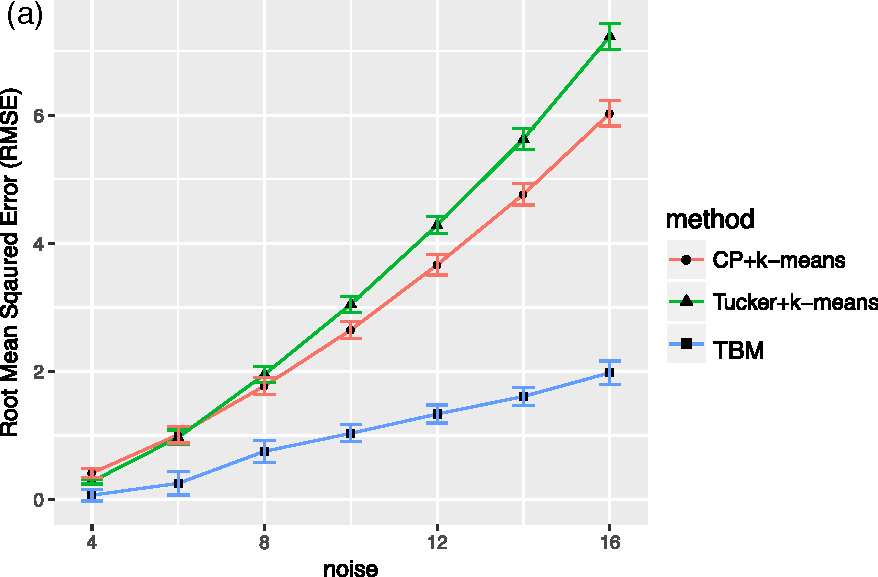
\includegraphics[width=.38\textwidth]{figures/clustering_404040_sparse}
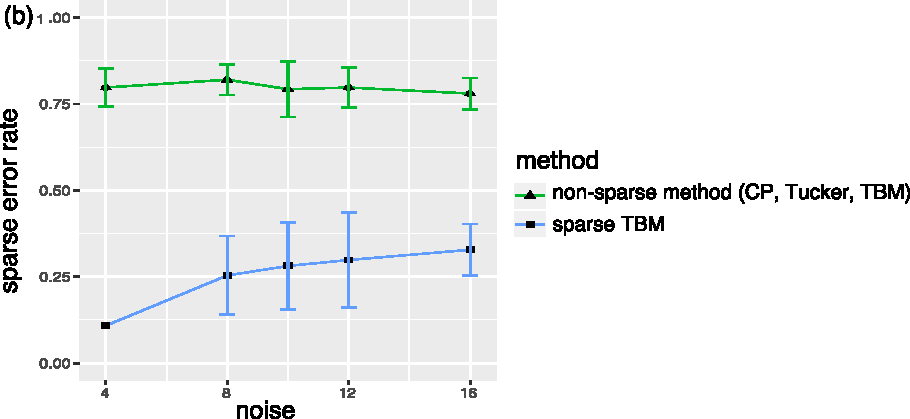
\includegraphics[width=.55\textwidth]{figures/clustering_correct_sparse}
\end{center}
\caption{(a) estimation error and (b) sparse error rate against noise for sparse tensors of dimension $(40,40,40)$ when $\rho=0.8$. }\label{fig:sparse}
\end{figure}


\begin{table}[http]


	\centering	

	\begin{tabular}{c|c|c|c}
		\hline
		Dimensions &True clustering sizes&Noise&Estimated clustering sizes\\ 
$(d_1,d_2,d_3)$&$(R_1,R_2,R_3)$&$(\sigma)$&$(\hat R_1,\hat R_2,\hat R_3)$\\
		\hline
		%$(50,60,80)$&$(3,4,5)$&4&$(,\ ,\ )\pm (0,\ 0,\ 0)$\\
		%$(50,60,80)$&$(3,4,5)$&8&$(,\ ,\ )\pm (0,\ 0.02,\ 0.06)$ \\
		%$(50,60,80)$&$(3,4,5)$&12&$(,\ ,\ )\pm (0.06,\ 0.09,\ 0.11)$\\
		%$(50,60,80)$&$(4,5,10)$&4&$(,,,)\pm (0,0,0)$\\
		%$(50,60,80)$&$(4,5,10)$&8&$(3.94,3.96,3.96)\pm (0.03,0.03,0.03)$\\
		%$(50,60,80)$&$(4,5,10)$&12&$(3.08,3.12,3.12)\pm(0.10,0.10,0.10)$\\
		$(40,40,40)$&$(4,4,4)$&4&$({\bf 4},\ {\bf 4},\ {\bf 4})\pm (0,\ 0,\ 0)$\\
		$(40,40,40)$&$(4,4,4)$&8&$({\bf 3.94},\ {\bf 3.96},\ {\bf 3.96})\pm (0.03,\ 0.03,\ 0.03)$\\
		$(40,40,40)$&$(4,4,4)$&12&$(3.08,\ 3.12,\ 3.12)\pm (0.10,0.10,0.10)$\\
		\hline
		$(40,40,80)$&$(4,4,4)$&4&$({\bf 4},\ {\bf 4},\ {\bf 4})\pm (0,\ 0,\ 0)$\\
		$(40,40,80)$&$(4,4,4)$&8&$({\bf 4},\ {\bf 4},\ {\bf 4})\pm (0,\ 0,\ 0)$\\
		$(40,40,80)$&$(4,4,4)$&12&$({\bf 3.96},\ {\bf 3.96},\ 3.92)\pm (0.04,0.04,0.04)$\\
			\hline
		$(40,40,40)$&$(2,3,4)$&4&$({\bf 2},\ {\bf 3},\ {\bf 4})\pm (0,\ 0,\ 0)$\\
		$(40,40,40)$&$(2,3,4)$&8&$({\bf 2},{\bf \ 3},\ {\bf 3.96})\pm (0,\ 0,\ 0.03)$ \\
		$(40,40,40)$&$(2,3,4)$&12&$({\bf 2},\ {\bf 2.96},\ 3.60)\pm (0,\ 0.05,\ 0.09)$\\
\vspace{.1cm}
		%\hline
	\end{tabular}
		\caption{The simulation results for estimating $\mR=(R_1,R_2,R_3)$. Bold number indicates no significant difference between the estimate and the ground truth, based on a $z$-test with a level $0.05$.}\label{tab:rank}
\end{table}

\begin{table}[H]
	\centering
\resizebox{\columnwidth}{!}{
	\begin{tabular}{c|c|c|c|c}
Tissues & Over-expressed genes  &Block-means&Under-expressed genes&Block-means \\
\hline
Cluster 1&GFAP, MBP&10.88&GPR6 , DLX5 , DLX6 , NKX2-1&-8.40\\
\hline
Cluster 2 &GFAP, MBP&5.98 &CDH9, RXFP1, CRH, ARX, CARTPT, DLX1,FEZF2  &-9.49\\
\hline
\multirow{2}{*}{Cluster 3 }&\multirow{2}{*}{GFAP, MBP} &\multirow{2}{*}{8.34}&AVPR1A, CCKAR, CHRNB4, CYP19A1, HOXA4 , LBX1, SLC6A3&-8.45\\
 &&& TBR1, SLC17A6, SLC30A3& -8.17\\
 \hline
\multirow{2}{*}{Cluster 4}&\multirow{2}{*}{ GFAP, MBP} &\multirow{2}{*}{8.83}&AVPR1A, CCKAR, CHRNB4, CYP19A1, HOXA4 , LBX1, SLC6A3&-8.40 \\
 &&&DAO   EN2   EOMES& -6.57\\
\end{tabular}
}
\caption{\small Top expression blocks from the multi-tissue gene expression analysis. The tissue clusters are described in Supplementary Section~\ref{sec:data}.}\label{tab:gene}
\end{table}

\begin{table}[H]
	\centering
\resizebox{\columnwidth}{!}{
	\begin{tabular}{c|c|c}
Countries & Countries  & Relation types  \\
\hline
Cluster 1&Clusters 4 and 5&reltreaties, booktranslations, relbooktranslations, relexports, exports3\\
\hline
Clusters 1 and 4& Cluster 5&relintergovorgs, relngo, intergovorgs3, ngoorgs3\\
\hline
Cluster 3&Clusters 1, 4, and 5&commonbloc0, blockpositionindex\\
\hline
Clusters 1 and 3&Clusters 4 and 5&\multirow{3}{*}{timesinceally, independence}\\
Cluster 1 & Cluster 3&\\
Cluster 4 & Cluster 5&\\
\hline
\multirow{3}{*}{Cluster 4}&\multirow{3}{*}{Cluster 5}&treaties, conferences, weightedunvote, unweightedunvote, intergovorgs, ngo,\\
& &officialvisits, exportbooks, relexportbooks, tourism,\\
&&reltourism, tourism3, exports, militaryalliance, commonbloc2
\vspace{.1cm}
\end{tabular}
}
\caption{\small Top blocks from the \emph{Nations} data analysis. The countries clusters are described in Supplementary Section~\ref{sec:data}.}\label{tab:rel}
\end{table}


%\begin{table}[http]
%	\centering
%	\resizebox{\textwidth}{20mm}{
%	\begin{tabular}{|c|c|c|c|c|c|c|c|c|c|c|}
%		\hline
%		$n_1$&$n_2$&$n_3$&$d_1$&$d_2$&$d_3$&noise&overall accuracy&estimated $d_1$&estimated $d_2$&estimated $d_3$\\ \hline
%		40&40&40&3&5&4&4&$\mathbf{1}$&3(0)&5(0)&4(0)\\
%		40&40&40&3&5&4&8&0.74&3(0)&4.76(0.0610)&3.98(0.02)\\
%		40&40&40&3&5&4&12&0.02&2.8(0.0571)&3.58(0.1072)&3.3(0.0915)\\
%		40&40&40&4&4&4&4&$\mathbf{1}$&4(0)&4(0)&4(0)\\
%		40&40&40&4&4&4&8&0.88&3.94(0.0339)&3.96(0.0280)&3.96(0.0280)\\
%		40&40&40&4&4&4&12&0.04&3.08(0.0983)&3.12(0.1016)&3.12(0.0975)\\
%		40&40&80&4&4&4&4&$\mathbf{1}$&4(0)&4(0)&4(0)\\
%		40&40&80&4&4&4&8&1&4(0)&4(0)&4(0)\\
%		40&40&80&4&4&4&12&0.78&3.9(0.0429)&3.92(0.0388)&3.96(0.04)\\
%		\hline
%	\end{tabular}}
%	\caption{The simulation results across 50 tensors each time from estimating the $d_1,d_2,d_3$.}
%	\label{t2}
%\end{table}

%\begin{table}
%	\centering
%	\begin{tabular}{|c|c|c|c|c|c|c|}
%		\hline
%		$n_1$&$n_2$&$n_3$&noise&CER(mode 1)&CER(mode 2)&CER(mode3)\\ \hline
%		40&40&40&4&$\mathbf{0(0)}$&$\mathbf{0(0)}$&$\mathbf{0(0)}$\\
%		40&40&40&8&$\mathbf{0(0)}$&0.0136(0.0226)&0.0005(0.0036) \\
%		40&40&40&12&0.0365(0.0789)&0.12(0.0878)&0.0802(0.1009)\\
%		40&45&50&4&$\mathbf{0(0)}$&$\mathbf{0(0)}$&$\mathbf{0(0)}$\\
%		40&45&50&8&$\mathbf{0(0)}$&0.0027(0.0121)&$\mathbf{0(0)}$\\
%		40&45&50&12&0.0158(0.0489)&0.0641(0.0629)&0.0336(0.0647)\\
%		\hline
%	\end{tabular}
%	\caption{The CERs over 50 simulated tensors ($d_1=3, d_2=5, d_3=4$) each time.}
%	\label{t3}
%\end{table}


%\begin{tabular}[ccc]
 %"China"   "Cuba" "Poland"   "USSR" & UK/USA& 4
%\end{tabular}

%\begin{itemize}
%\item 2 (Exports): reltreaties, booktranslation, relbooktranslations, relexports, exports3
%\item 4 (Independence): "timesinceally"  "independence" 
%\item 5 (NGO): relintergovorgs"          "relngo"   "intergovorgs3"        "ngoorgs3" 
%\item 6 (edunvote)"treaties"      "conferences"   "weightedunvote" "unweightedunvote" "intergovorgs"              "ngo" 
%\item 9 (tourist):"officialvisits"      "exportbooks"   "relexportbooks"          "tourism" "reltourism"         "tourism3"          "exports" "militaryalliance" 
 %"commonbloc2" 

%\end{itemize}

\section{Time complexity}
The total cost of our Algorithm~\ref{alg:B} is $\tO(d)$ per iteration, where $d=\prod_k d_k$ denotes the total number of tensor entries. The per-iteration computational cost scales linearly with the sample size, and this complexity is comparable to the classical tensor methods such as CP and Tucker decomposition. More specifically, each iteration of Algorithm~\ref{alg:B} consists of updating the core tensor $\tC$ and $K$ membership matrices $\mM_k$'s. The update of $\tC$ requires $\tO(d)$ operations and the update of $\mM_k$ requires $\tO(R_k{d\over d_k})$ operations. Therefore the total cost is $\tO(d+d\sum_k {R_k\over d_k})$. %We further report the computational time in Supplementary Section~\ref{sec:data}.


\section{Additional information for real data analysis}\label{sec:data}
{\bf Multi-tissue gene expression.} The gene expression data we analyzed is part of the GTEx v6 datasets (\url{https://www.gtexportal.org/home/datasets}). We cleaned and preprocessed the data following the steps in~\cite{wang2017three}. We focused on the 13 brain tissues, 193 individuals, and 362 annotated genes provided by Atlax of the Developing Human Brain (\url{http://www.brainspan.org/ish}). After applying the $\ell$-0 penalized TBM to the mean-centered data tensor, we identified the following four clusters of tissues:
\begin{enumerate}[label=-, leftmargin=*]
\item Cluster 1: Substantia nigra, Spinal cord (cervical c-1)
\item Cluster 2: Cerebellum, Cerebellar Hemisphere
\item Cluster 3: Caudate (basal ganglia), Nucleus accumbens (basal ganglia), Putamen (basal ganglia)
\item Cluster 4: Cortex, Hippocampus, Anterior cingulate cortex (BA24), Frontal Cortex (BA9), Hypothalamus, Amygdala
\end{enumerate}

We found that most tissue clusters are spatially restricted to specific brain regions, such as the two cerebellum tissues (cluster 2), three basal ganglia tissues (cluster 3), and the cortex tissues (cluster 4). Supplementary Table~\ref{tab:gene} reports the associated gene cluster for each tissue cluster. Because our method attaches importance to blocks by the absolute mean estimates, our method is able to detect both over- and under-expression patterns. Blocks with highly positive means correspond to over-expressed genes, whereas blocks with highly negative means correspond to under-expressed genes. 


{\bf Nations dataset.} This is a $14 \times 14 \times 56$ binary tensor consisting of $56$ political relations of $14$ countries between 1950 and 1965~\cite{nickel2011three}. The tensor entry indicates the presence or absence of a political action, such as ``treaties'', ``sends tourists to'', between the nations. We applied the $\ell$-0 penalized TBM to the binary-valued data tensor, and we identified the following five clusters of countries:
\begin{enumerate}[label=-, leftmargin=*]
\item Cluster 1: Brazil, Egypt, India, Israel, Netherlands
\item Cluster 2: Burma, Indonesia, Jordan
\item Cluster 3: China, Cuba, Poland, USSA
\item Cluster 4: USA
\item Cluster 5: UK
\end{enumerate}
Supplementary Table~\ref{tab:rel} reports the cluster constitutions for top blocks. Because the tensor entries take value on either 0 or 1, the top blocks mostly have mean one. 


\end{appendices}
\bibliographystyle{unsrt}
\bibliography{tensor_wang}

\end{document}

\begin{comment}
\begin{align}
\FnormSize{}{\hat \Theta-\trueT}&\leq 2\sup_{\mu\in\tD(R)} \sup_{\mu'\in \tD(R)} \Big\langle {\mu-\mu'\over \FnormSize{}{\mu-\mu'}}, \tE \Big\rangle\\
&\leq \sup_{\mu\in \tD(R)}\sup_{\mu'\in \tD(R)\cap \mB_2(\mu)}\langle \mu', \tE  \rangle\\
&\leq \sup_{\mu \in \tD(R)} 6^R{d \choose R}
\end{align}
\begin{align}
\sup_{\mu\in (\tP-\tP')\cap \mB^d_2}\langle \mu ,\tE\rangle&\leq \sup_{\mu\in \tD()\cap\mB^d_2}\sup_{\tP} \langle \mu, \tE\rangle\\
&\leq \sup_{|\ms|= R^2}\sup_{\mu\in\mB_2^{\ms}}\langle \mu, \tE\rangle\\
&\leq2\sigma \log\left(6^{R^2}{d \choose R^2}\right)\\
&\leq 2\sigma R^2+....
\end{align}
with probability at least $1-\exp(R^2)$
\end{proof}
\subsection{Proof of Theorem~\ref{thm:main}}
To study the performance of the least-square estimator $\hat \Theta$, we need to introduce some additional notations. We view the membership matrix $\mM_k$ as an onto function $\mM_k\colon [d_k]\mapsto [R_k]$, and with a little abuse of notation, we still use $\mM_k$ to denote the mapping function. Correspondingly, we use $\mM_k(i_k)$ to denote the cluster label for the element $i_k\in[d_k]$, and $\mM^{-1}_k(r_k)$ the group of elements in cluster $r_k\in[R_k]$.

To simplify notation, we define $\mi=(i_1,\ldots,i_K)$, $\mr=(r_1,\ldots,r_K)$, and $\mM^{-1}(\mi)=\mM_1^{-1}(r_1)\times \cdots \times \mM^{-1}_K(r_K)$. 
The parameter space $\tP$ can be equivalently written as
\begin{align}
\tP=&\big\{ \Theta\in\mathbb{R}^{d_1\times \cdots\times d_K}\colon \Theta_{\mi}=\tC_{\mr} \text{ for }\mi \in\mM^{-1}(\mr)\text{ and a core tensor $\tC\in\mathbb{R}^{R_1\times \cdots \times R_K}$} \big\}.\notag
\end{align}
That is, the mean signal tensor $\Theta$ is a piecewise constant with respect to the blocks in the Cartesian product of the mode-$k$ clusters, $\mM^{-1}(\mi)$, for all $\mr \in[R_1]\times \cdots\times [R_K]$. 

The estimate $\hat \Theta$ consists of two components: the mean parameter $\tC$ and the clustering (structure) parameter $ \mM\colon [d_1]\times \cdots [d_K]\mapsto [R_1]\times \cdots \times [R_K]$. We introduce an intermediate estimate 
\[
\bar \Theta =\mathbb{E}(\hat \Theta|\hat \mM)=\mathbb{E}(\hat \tC\times_1 \hat \mM_1\times\cdots \times_K \hat \mM_K|\hat \mM),
\] 
where the expectation is taken with respect to the $\hat \tC$ (which is a function of the data $\tY$). Note that, given the structure estimate $\hat \mM$, the mean estimate $\hat \tC$ is simply the sample average of $\tY$ within the blocks defined by $\hat \mM$. Therefore, 
%\begin{align}
%\bar \Theta=\mathbb{E}(\hat \tC|\hat \mM)\times_1\hat \mM_1\times\cdots \times_k \hat \mM_K&=\tC\times_1 (\mB_1\hat \mM_1)\cdots \times_K(\mB_K\hat \mM_K)\\
%&=\KeepStyleUnderBrace{(\tC\times_1\mB_1\times \cdots \times_K \mB_K)}_{\bar \tC}\times_1\hat \mM_1\times_2 \cdots \times_K\hat \mM_K
%\end{align}
%where $\mB_k=\mM_k\hat \mM'_k(\hat \mM_k\hat \mM'_k)^{-1}$ is the (row-normalized) confusion matrix between $\mM_k$ and $\mM'_k$, for all $k\in[K]$.
Note that $\hat \Theta$ is the minimizer of $\FnormSize{}{\Theta -\tY}$. By Lemma 1, 
\[
\FnormSize{}{\hat \Theta -\trueT}\leq 2 \langle \hat \Theta-\bar\Theta,\ \tY-\trueT \rangle+2\FnormSize{}{\hat \Theta-\bar\Theta} \delta +2 \delta^2
\]
where $\delta=|\langle {\bar \Theta -\trueT\over  \FnormSize{}{\bar \Theta-\trueT}}, \tY-\trueT  \rangle|.$

\begin{lemma} With probability at least $1-\exp(\prod_k R_k + \sum_k d_k \log R_k)$
\[
\langle\hat \Theta -\bar \Theta, \tY-\trueT\rangle\leq C_1\sigma^2 \left( \prod_k R_k+\sum_k R_k\log d_K\right),
\]
holds uniformly over $\hat \mM$. 
\end{lemma}

\begin{proof}
 For any fixed index $\mi\in[d_1]\times \cdots [d_K]$. Suppose that the index $\mi$ belongs to the block $\mr$ according to $\hat \mM$; i.e. $\hat \mM(\mi)=\mr$. Then
\[
\hat \Theta_{\mi}={1\over |\hat \mM^{-1}(\mr)|} \sum_{\mj\in\hat \mM^{-1}(\mr)}\tY_{\mj}.
\]
By the definition of $\bar \Theta=\mathbb{E}(\hat \Theta|\hat \mM)$, we have
\begin{align}
\hat \Theta_{\mi}-\bar \Theta_{\mi}&={1\over |\hat \mM^{-1}(\mr)|} \sum_{\mj\in\hat \mM^{-1}(\mr)}\left(\tY_{\mj}-\mathbb{E}(\tY_{\mj})\right)\\
&={1\over| \hat \mM^{-1}(\mr)|} \sum_{\mj\in\hat \mM^{-1}(\mr)}\tE_{\mj}
\end{align}
Therefore, 
\[
\langle \hat \Theta-\bar \Theta, \tY-\trueT\rangle=\sum_{\mr}\left({1\over \sqrt{|\hat \mM^{-1}(\mr)|}} \sum_{\mj\in\hat \mM^{-1}(\mr)}\tE_{\mj}\right)^2
\]
Note that $\tE_{\mj}$ follows the independent sub-Gaussian-$\sigma^2$ assumption. Hence
\[
{1\over \sqrt{|\hat \mM^{-1}(\mr)|}} \sum_{\mj\in\hat \mM^{-1}(\mr)}\tE_{\mj}
\]
 s sub-Gaussian with-$\sigma^2$. There are $\prod_k R_k$ choices of $\mr$. By union bound, with probability at least $1-\exp(\prod_k R_k+\sum_k d_k\log R_k)$
\[
|\hat \Theta-\bar\Theta, \tY-\trueT| \leq C_1 \sigma^2 \left(\prod_k R_k+\sum_k d_k \log R_k\right)
\]
uniformly holds for all $\hat \mM$.
\end{proof}
\begin{lemma} With probability at least $1-\exp(\sum_k d_k \log R_k)$,
\[
\Big \langle{ \bar \Theta -\trueT \over \FnormSize{}{\bar \Theta -\trueT}},\ \tY-\trueT \Big \rangle\leq C_2\sigma\left(\prod_k d_k+\sum_k d_k \log R_k \right)^{1/2}.
\]
\end{lemma}
\begin{proof}
Define 
\[
\tB=\{ \entry{\tC}: \}
\]
\end{proof}

\begin{lemma} With probability at least $1-\exp(\sum_k R_k+\sum_k R_k\log d_k)$,
\[
\FnormSize{}{\hat \Theta -\bar \Theta}\leq C_3\sigma\left(\prod_k R_k+\sum_k d_k \log R_k \right)^{1/2}.
\]
\end{lemma}

\begin{proof} From the proof of Lemma 1, we have
\[
\FnormSize{}{\hat \Theta-\bar \Theta}^2=\sum_{\mr}{1\over |\mM^{-1}(\mr)|}\left(\sum_{\mj \in \hat \mM^{-1}(\mr)}\tE_{\mj}\right)^2.
\]
Note that ${{1\over \sqrt{|\mM^{-1}(\mr)|}}\sum_{\mj\in \hat \mM^{-1}(\mr)}\tE_{\mj}$ follows independent Gaussian-$\sigma$. (same as Lemma 1?) So
\[
\FnormSize{}{\hat \Theta-\bar \Theta} \leq C \sigma\left(\prod_k R_k+\sum_k d_k \log R_k\right)
\]
uniformly over $\mM$.
\end{proof}

\begin{lemma} Let $\ma, \mb\in\mathbb{R}^d$ be two vectors and $\normSize{}{\cdot}$ the Euclidean norm in $\mathbb{R}^2$. If $\normSize{}{\mb}\leq \normSize{}{\ma}$, then the following hold for any $\mx\in\mathbb{R}^d$:
\[
\normSize{}{\ma-\mb}\leq 2 \langle \mx,\ma\rangle  + 2\normSize{}{\mx}\delta+2\delta^2,\quad \text{with}\quad \delta=\Big|\large \Big\langle{\ma-\mb-\mx\over\normSize{}{\ma-\mb-\mx}},\ \ma \Big\rangle\Big|
\]
\end{lemma}
Let $d=\prod_k d_k$ and $R=\prod_k R_k$. We define $\tD(s)$ to be the set of $d$-dimensional vectors with at most $s$ distinct entry values. 
By identifying the tensors in $\tP$ as $d$-dimensional vectors, we have $\tP\subset \tD^d(R)$.


Now consider the least-square estimator
\[
\hat \Theta=\argmin_{\Theta\in\tP}\{-2\langle \tY, \Theta\rangle+\FnormSize{}{\Theta}^2 \}=\argmin_{\Theta\in\tP}\{\FnormSize{}{\tY-\Theta}^2 \}.
\]
Based on Proposition~\ref{prop:bound}, we have
\[
\FnormSize{}{\hat \Theta-\trueT} \leq 2\sup_{\mu\in (\tP-\tP') \cap \mB^d_2}\langle \mu ,\tE\rangle,
\]
where $(\tP-\tP')=\{\mu-\mu'\colon \mu, \mu'\in\tP\}$ and $\mB^{d}_2$ denotes the Euclidean unit ball in dimension $d$. Based on the definition we have
\[
(\tP-\tP')\subset \tD^d(R^2).
\]

(to be finished...)
\begin{align}
\FnormSize{}{\hat \Theta-\trueT}&\leq 2\sup_{\mu\in\tD(R)} \sup_{\mu'\in \tD(R)} \Big\langle {\mu-\mu'\over \FnormSize{}{\mu-\mu'}}, \tE \Big\rangle\\
&\leq \sup_{\mu\in \tD(R)}\sup_{\mu'\in \tD(R)\cap \mB_2(\mu)}\langle \mu', \tE  \rangle\\
&\leq \sup_{\mu \in \tD(R)} 6^R{d \choose R}
\end{align}
\begin{align}
\sup_{\mu\in (\tP-\tP')\cap \mB^d_2}\langle \mu ,\tE\rangle&\leq \sup_{\mu\in \tD()\cap\mB^d_2}\sup_{\tP} \langle \mu, \tE\rangle\\
&\leq \sup_{|\ms|= R^2}\sup_{\mu\in\mB_2^{\ms}}\langle \mu, \tE\rangle\\
&\leq2\sigma \log\left(6^{R^2}{d \choose R^2}\right)\\
&\leq 2\sigma R^2+....
\end{align}
with probability at least $1-\exp(R^2)$

For fixed $\mM_k$'s, $\tC$ is a linear space of dimension no greater than $R^2$. 
%Let $\tD$ denote a subset of $\mathbb{R}$ with $\prod_k R_k$ finite elements. We also call $\tD$ an alphabet with $|\tD|=\prod_k$. Then
%\[
%\tP\subset \{\Theta\colon \Theta\in \tD^{d_1\times \cdots d_K}\}.
%\]
\end{comment}